%% by Michael Shell
%% Edited by Rodrigo Almeida
%%
%% This work is distributed under the LaTeX Project Public License (LPPL)
%% ( http://www.latex-project.org/ ) version 1.3, and may be freely used,
%% distributed and modified. A copy of the LPPL, version 1.3, is included
%% in the base LaTeX documentation of all distributions of LaTeX released
%% 2003/12/01 or later.
%% Retain all contribution notices and credits.

\documentclass[10pt,journal,compsoc]{IEEEtran}

\hyphenation{op-tical net-works semi-conduc-tor}


\usepackage{hyperref}
\usepackage{biblatex}
\usepackage{graphicx}
\usepackage{listings}
\usepackage{multirow}
\usepackage{tabularx}
\usepackage{caption}
\usepackage{booktabs}

\graphicspath{{images/}}

\addbibresource{references.bib}

\begin{document}
% paper title
% Titles are generally capitalized except for words such as a, an, and, as,
% at, but, by, for, in, nor, of, on, or, the, to and up, which are usually
% not capitalized unless they are the first or last word of the title.
% Linebreaks \\ can be used within to get better formatting as desired.
% Do not put math or special symbols in the title.
% \title{Transparency in AI - Decision-Making with Explainable AI (XAI)}
\title{Why Explain a decision made by AI? Explainable AI (XAI)}

% author name
\author{Rodrigo Almeida% <-this % stops a space
}

% The paper headers
\markboth{Research Methods in Computing \& IT - Literature Review}%
{}

\IEEEtitleabstractindextext{
    \begin{abstract}
        In this paper, I will review the literature relating to transparency for decisions made by artificial intelligence (AI). As AI advances, not only our dependence on AI models are increasing but also a need for understanding how such results and decisions were made by the model. Due to the complexity of AI, Explainable Artificial Intelligence (XAI) has become a great choice, bringing more clarity, where outputs can be explained reducing bias and bringing transparency to the decision-making process, as opposed to "Black Box" algorithms that we cannot explain why or how the AI arrived in such a conclusion/classification/decision, it outputs directly from data, and not even who developed such algorithms are able to explain how the model arrived in such result. 
        
      
    \end{abstract}
}

% make the title area
\maketitle

\section{Introduction}
\label{sec:introduction}

\IEEEPARstart{E}xplainable AI is emerging, and with it, the concerns from scientists, the general public and policymakers are also on the rise. As artificial intelligence, machine learning and deep learning are becoming integrated into applications, decisions from such models can carry consequences for a person and society, changing the focus from accuracy to the necessity of being able to explain and clarify how these decisions were made.\cite{analytical-review} As we are becoming more dependent and relying hugely on intelligent machines, whether it is email filters, AI helping with medical diagnoses or self-driving cars, machine learning is being used across almost all sectors. Such growth in these technologies only highlights the importance of understanding the interpretability of the outcome generated by it. This is the main motivation for explainable artificial intelligence.\cite{doshivelez2017rigorous} 
The impact of the outcome will vary based on the field. A wrong prediction for computing and business might lead to misleading recommendations, potentially affecting the revenue of such businesses, however wrong predictions in critical sectors like healthcare could put human life at risk. Opening the "black box" is incredibly important, not just for social acceptance but also for regulatory purposes. Understanding how AI systems reach their conclusions is crucial in ensuring accountability, transparency, and ethical use of these technologies, making it essential for both public trust and regulatory compliance.\cite{analytical-review}

In \autoref{fig:xaiGraphic} we can easily understand the main differences between the "Black Box" and XAI.\cite{xai-concept}

\begin{figure}[h]
    \centering
    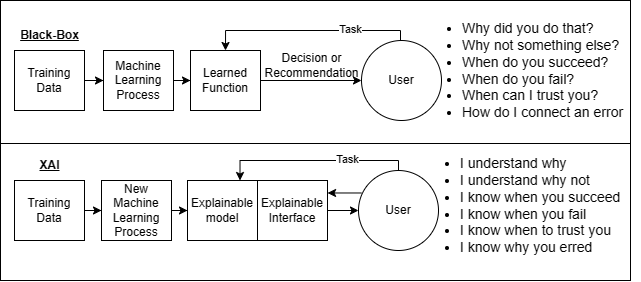
\includegraphics[scale=0.37]{xaiGraphic.png}
    \caption{XAI Concept}
    \label{fig:xaiGraphic}
\end{figure}

\section{Definitions}

Explainable AI (XAI) is a field focused on increasing human understanding of AI systems. Although terms like transparency, interpretability, and explainability are frequently used together, they can have different meanings, there are differences between these theories.\cite{xai-ml}

\begin{itemize}
    \item {Transparency}: a model deemed transparent is one that can be understood easily on its own. It is the opposite of a "black box", indicating that the inner workings of the model are understandable\cite{transparency}.
    \item {Interpretability}: It is the ability to explain concepts that are complex or result in a way that humans will easily understand\cite{gilpin2019explaining}.
    \item {Explainability}: it is the concept that provides explanations as a bridge between AI systems and humans. It involves the ability to create AI systems that are not only accurate but also people can understand.\cite{gilpin2019explaining}.
\end{itemize}

\section{Overview of Explainable AI Algorithms}
Researchers have developed many algorithms to explain AI systems. These explanations could be categorized into two primary groups: self-interpretable models refer to the algorithm model itself or a representation of the algorithm that can be directly read and comprehended by a human. In this case, the model itself serves as the explanation. On the other hand, post-hoc explanations are descriptions, explanations, or models of the algorithm often produced by separate software tools. These tools aim to provide an understanding of how the algorithm operates. Post-hoc explanations are particularly useful for algorithms for which the inner workings are not fully transparent, as they can be employed to generate insights without requiring deep knowledge of the algorithm's internal mechanisms. Instead, they rely on querying the algorithm for outputs based on selected inputs.\cite{phillips2020four}.

\section{Future Work}


\section{Conclusion}


\appendices
\section{Proof of the First Zonklar Equation}


\section{}


% references section
\printbibliography

\end{document}